% Made up for the tikra benchmark.
\pgfplotsset{compat=1.18}
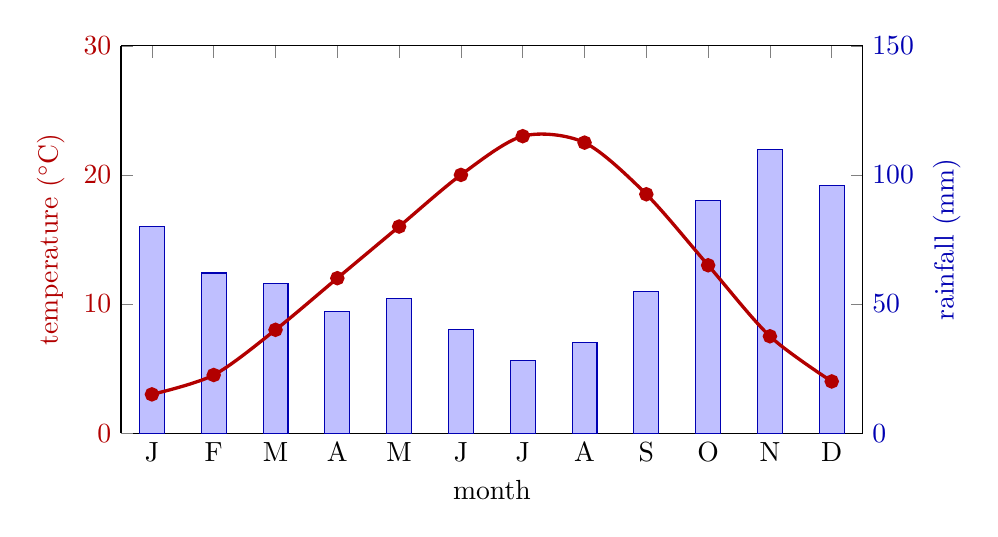
\begin{tikzpicture}
  \pgfplotsset{every axis/.style={width=11cm, height=6.5cm, xmin=0.5, xmax=12.5, xtick={1,...,12},
    xticklabels={J,F,M,A,M,J,J,A,S,O,N,D}}}
  \begin{axis}[axis y line*=right, ymin=0, ymax=150, ylabel={rainfall (mm)}, xlabel={month},
      ylabel style={blue!70!black}, yticklabel style={blue!70!black}]
    \addplot[ybar, bar width=9pt, fill=blue!25, draw=blue!70!black]
      coordinates {(1,80) (2,62) (3,58) (4,47) (5,52) (6,40) (7,28) (8,35) (9,55) (10,90) (11,110) (12,96)};
  \end{axis}
  \begin{axis}[axis y line*=left, axis x line=none, ymin=0, ymax=30, ylabel={temperature ($^\circ$C)},
      ylabel style={red!70!black}, yticklabel style={red!70!black}]
    \addplot[red!70!black, very thick, mark=*, smooth]
      coordinates {(1,3) (2,4.5) (3,8) (4,12) (5,16) (6,20) (7,23) (8,22.5) (9,18.5) (10,13) (11,7.5) (12,4)};
  \end{axis}
\end{tikzpicture}
